\documentclass[tikz,border=8pt]{standalone}
\usetikzlibrary{arrows.meta,positioning,calc}
\begin{document}
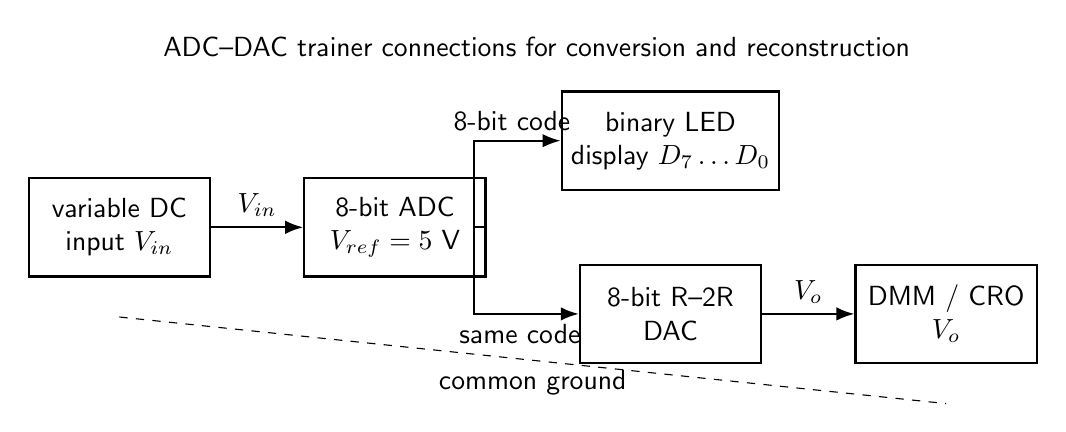
\begin{tikzpicture}[font=\sffamily, box/.style={draw,thick,minimum width=2.3cm,minimum height=1.25cm,align=center}, arr/.style={-{Latex[length=2.3mm]},thick}]
  \node[box] (src) at (0,2.2) {variable DC\\input $V_{in}$};
  \node[box] (adc) at (3.5,2.2) {8-bit ADC\\$V_{ref}=5$ V};
  \node[box] (led) at (7.0,3.3) {binary LED\\display $D_7\ldots D_0$};
  \node[box] (dac) at (7.0,1.1) {8-bit R--2R\\DAC};
  \node[box] (meter) at (10.5,1.1) {DMM / CRO\\$V_o$};
  \draw[arr] (src) -- node[above]{$V_{in}$} (adc);
  \draw[arr] (adc) -- ++(1.0,0) |- node[pos=.72,above]{8-bit code} (led);
  \draw[arr] (adc) -- ++(1.0,0) |- node[pos=.72,below]{same code} (dac);
  \draw[arr] (dac) -- node[above]{$V_o$} (meter);
  \draw[dashed] ($(src.south)+(0,-.5)$) -- ($(meter.south)+(0,-.5)$) node[midway,below]{common ground};
  \node[above] at (5.3,4.25) {ADC--DAC trainer connections for conversion and reconstruction};
\end{tikzpicture}
\end{document}
